% file build.tex
\documentclass[12pt]{report}
\usepackage{geometry}
 \geometry{
 a4paper,
 left=20mm,
 right=20mm,
 top=20mm,
 bottom=20mm,
 }
\usepackage{abc}
\usepackage{pdfpages}
\usepackage{titlesec}


\begin{document}

%%%
%%% REDEFINE CHAPTER AND SECTION APPEARANCE
\titleformat
{\chapter} % command
[display] % shape
{\bfseries\Huge} % format
{} % label
{0.5ex} % sep
{
    \rule{\textwidth}{1pt}
    \vspace{1ex}
    \centering
} % before-code
[
\vspace{-2.0ex}%
\rule{\textwidth}{1pt}
] % after-code
 
 
\titleformat
{\section}
[display]
{\bfseries\huge\itshape}
{}
{0.5em}
{
	\centering
}
[]

\titlespacing{\chapter}{12pc}{-10ex}{3ex}

\titlespacing{\section}{12pc}{-10ex}{3ex}
%%%
%%%

% cover page	

\includepdf{../images/cover_fixed.pdf}
	
% table of contents
%\begin{center}
%
\includegraphics[width=4cm]{../images/contents}
%\end{center}
\tableofcontents

\chapter{Jigs}
\begin{center}
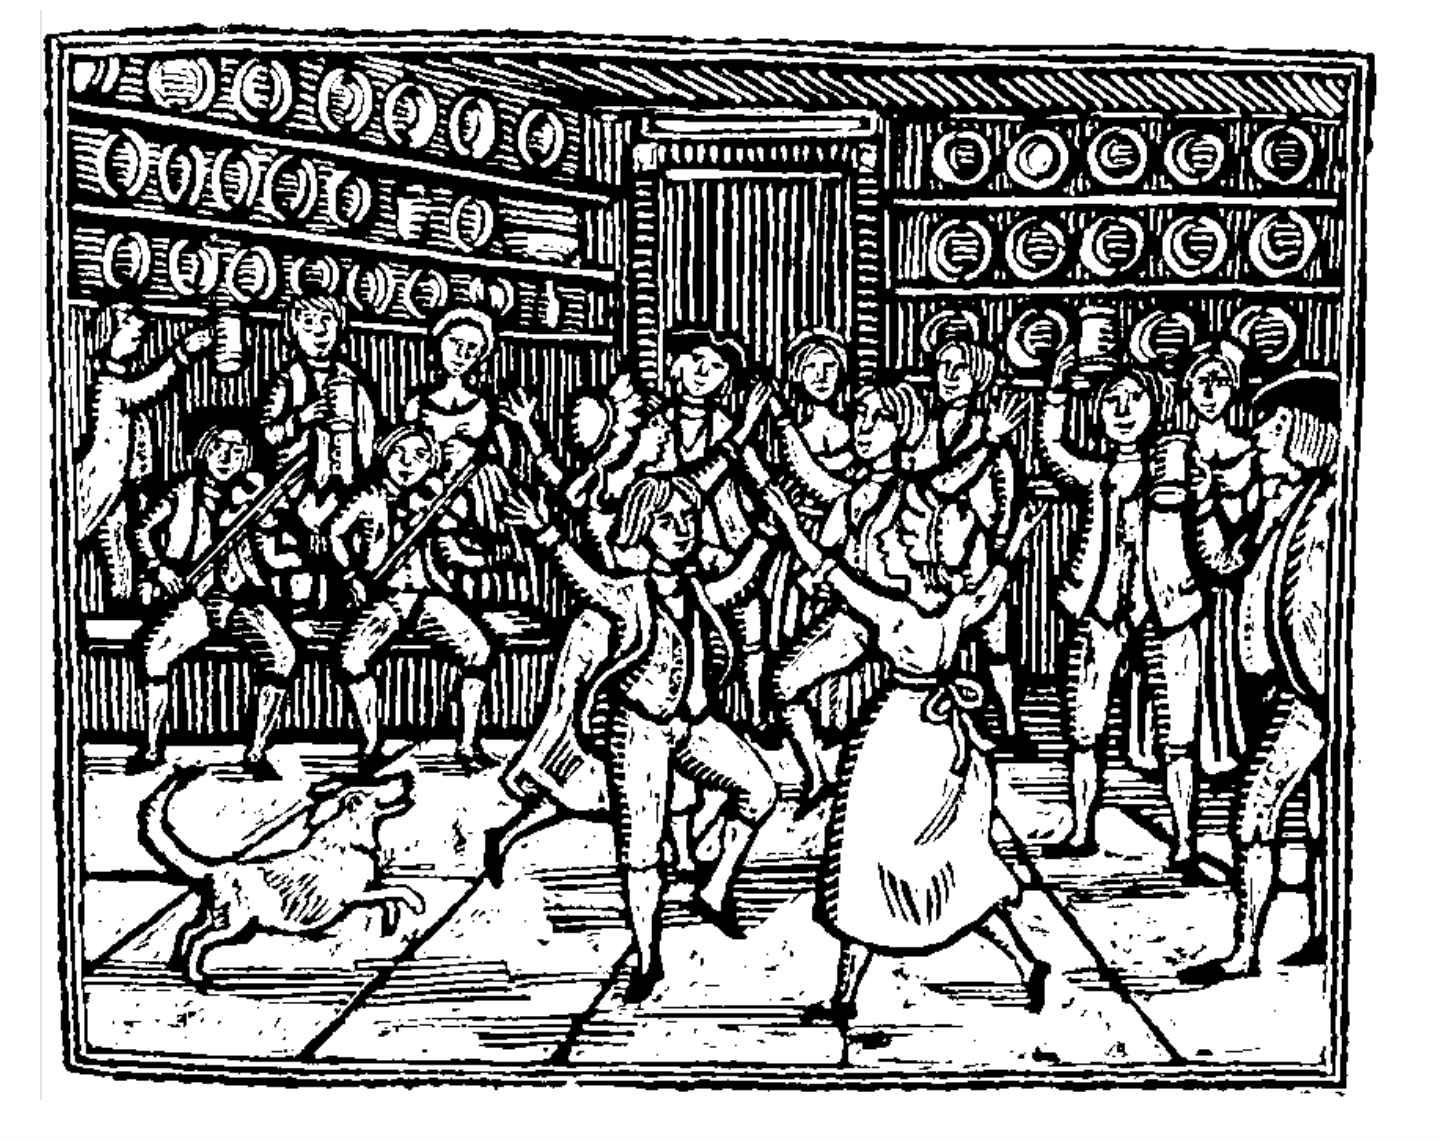
\includegraphics[width=8cm]{../images/jigs}
\end{center}

\section{Zycanthos}
\begin{abc}[name=Zycanthos]
X: 1
T: Zycanthos
R: jig
M: 6/8
L: 1/8
K: Amin
|:"Am" a2 a gag | "Am"e2 aagg | "Am"ecc BcB | "F"AFF F2 F |
"Am"EAB cBA | "F"FAB cBA | "G"B2 B edB| "Em"Bcd "Am"cBA :|
|: "AmE" EAB cBA | "F"FAB cBA | "G"B2 B edB | "Em"Bcd cBA |
"Am"EAB cBA | "F"FAB cBA | "G"B2 B edB |1 "Am"B2 A2 "F"F2 :|2"Am"B2A2 Bc ||
|: "Dm"d2 d-d2 c |"Dm" d c2 B2 A | "Dm"d2-d2 c d |"Em" B3 A3 |
"Dm"d2 d-d2 c | "Dm"d c2 B2 A | "Dm"d d-d2 c d | "Em"e3 ecA :|
\end{abc}

\begin{abc}[name=Jig_in_A]
X: 2
T: Jig in A
R: jig
M: 6/8
L: 1/8
K: Amin
|:"Am"EAA AGA|"G"Bdd dcd|"Am"eae "Em"dBG|"Am"ABA "F"AGF|
"Am"EAA AGA|"G"Bdd dcd|"Am"eae "Em"dBG|1 "Am"BAA A2F:|2 "Am"BAA ABd||
|:"A"eaa e3|"A"eaa bag|"A"eaa e3|"G"BGB dBG|
"A"eaa e3|"A"eaa bag|"A"eae "G"dBG|1 "A"BAA ABd:|2 "A"BAA A3|
\end{abc}

\begin{abc}[name=The_Peelers_Away_With_My_Daughter]
X: 3
T: The Peeler's Away With My Daughter
R: jig
M: 6/8
L: 1/8
K: Ador
|gf|:"Am"eAA ABd|ede "Em"g2 e|"G"dBG GAG|BGB dgf|
"Am"eAA ABd|ede "C"g2 a|"Em"g2 e "G"dBG|1 "Am"ABA A gf:|2 "Am"ABA A z "G"B||
|:"Am"eaa age|aga "Em"b2 a|"G"g2 a "Am7"gdB|"Gdim"gag "G"ged|
"Am"aba age|aga "G"b2 a|"Em"g2 e "G"dBG|1 "Am"ABA A z "G"B:|2"Am" ABA A3|
\end{abc}

\newpage
\section{From The New Country}
\begin{abc}[name=From_The_New_Country]
X: 1
T: From The New Country
R: jig
M: 6/8
L: 1/8
V:T1 name="Melody"   snm="M"
V:T2 name="Violin \n Accompaniment"  snm="V"
K: Edor
[V:T1]|:E/2F/2|"Em"GEE BEE|GEE BAG|"D"FDD ADD|d^cd AGF|
[V:T2]|:z| [B2E2] ([BG][B2E2]) ([BG]| [B2E2]) (EG2A)|[A2D2]([AF][A2D2]) ([AF]| [A2D2]) (F D2 ^D)|
[V:T1]"Em"GEE BEE|GEE (B2^c)|"Bm"d^cd "Bm7"AGF|"Em"GEE E2:|
[V:T2]e2 ([BG][B2E2]) ([BG]| [B2E2]) (E G,2 A,)|B,2 (FD2) (F| [E3G,3]) [e2B2E2]:|
[V:T1]|:B|"Em"B^c^d (e2f)|(e2f) "Bm7"edB|"Em"B^c^d (e2f)|"G"edB "D"d3|
[V:T2]|:z|(EGF) [B2E2] (G, &\ B3|A,2) (A,^A,2B,)|(EGF) [B2E2] (D &\B3|B,G,A,) [A3D3]|
[V:T1]"Em"B^c^d (e2f)|(e2f) edB|"Bm7"d^cd AGF|"Em"GEE E2:|]
[V:T2](EGF) [B2E2] (G, &\B3|A,2) (A,^A,2B,)|B,2 (FD2) (F|[E3G,3])[e2B2E2]:|]
\end{abc}

\begin{abc}[name=The_Blackthorn_Stick]
X: 2
T: The Blackthorn Stick
R: jig
M: 6/8
L: 1/8
V:T1 name="Melody"   snm="M"
V:T2 name="Violin \n Accompaniment"  snm="V"
K: Amaj
[V:T1]e|: "A"aga "D"faf | "A"ecA "D"BAF | "A"EAA "E7"GBB | "A"(Ac)c "E"B2 e |
[V:T2]z|: [e2c2] ([ec][e2d2]) ([de] | [e2c2]) ([ec][e2d2]) ([de] | [e3c3]) [B3E3] | [c3E3] [B2E2] z |
[V:T1]"F#m"aga "D"baf | "A"ecA "D"BAF | "A"EAA "E"GBB | "A"(cA)"D"A "A"A2 e :|
[V:T2] [e2c2] ([ec][e2d2]) ([de] | [e2c2]) ([ec][e2d2]) ([de] | [e3c3]) [B3E3] | ([c2E2]d) [c3E3] :|
[V:T1]|: "D"fee "A"aee| "D"fee "A"aee | "D"fee "F#m"agf | "A"edc "E"B2 e |
[V:T2]|: [fd] z2 [ec] z2| [fd] z2 [ec] z2| [fd] z2 [A3F3] | [A3E3] [G2B,2] z|
[V:T1]"F#m"aga "D"baf | "A"ecA "D"BAF | "A"EAA "E"GBB | "A"cA"D"A "A"A2 e :|
[V:T2][[e2c2] ([ec][e2d2]) ([de]| [e2c2]) ([ec][e2d2]) ([de]  | [e3c3]) [B3E3] | ([c2E2]d) [c3E3] :|
\end{abc}

\begin{abc}[name=Irish_Washerwoman]
X: 3
T: The Irish Washerwoman
R: jig
M: 6/8
L: 1/8
V:T1 name="Melody"   snm="M"
V:T2 name="Violin \n Accompaniment"  snm="V"
K: Gmaj
[V:T1]d/2c/2|:"G"BGG DGG|BGB dcB|"Am"cAA EAA|cAc "D"edc|
[V:T2]z|: [D2G,2] (([GB,][G2B,2])[GB,])| [D2G,2] [DB,] (([DB,]A,)G,) | [E2A,2] (([EC] [E2C2]) [EC]) | [E2A,2] (([EC] [D2C2]) [DC]) |
[V:T1]"G"BGG DGG|BGB dcB|"Am"cBc "D"Adc|1"G"BGG Gdc:|2"G"BGG Gga|]
[V:T2][D2G,2] (([GB,][G2B,2])[GB,])| [D2G,2] ([BD] [BD]AG)| [A2E2] (([AE][A2D2]) [AF]) | ([D2G,2] [GB,]) [G2B,2] z :| ([D2G,2] [GB,]) [G2B,2] z|]
[V:T1]|:"G"gdg gdg| gdg bag|"D"fdf fdf|fdf agf|
[V:T2]|: [B2G2] ([BG] [B2F2]) ([BF]| [B2E2]) ([BD] [BD]AG)| [A2D2] ([AD] [A2E2]) ([AE] | [A2=F2]) ([AF] [A2^F2]) z|
[V:T1]"C"egg "G"dgg|"C"cgg "G"Bgg|"Am"cBc "D"Adc|1"G"BGG Gdf:|2"G"BGG G3|]
[V:T2] [E2C2] z [D2B,2] z| [D2A,2] z [D2G,2] z | [E2A,2] (([EC] [D2C2]) [FC]) |1 ([D2G,2] [GB,]) [G2B,2] z :|2 ([D2G,2] [GB,]) [G2B,2] z |]
\end{abc}

\chapter{Reels}
\begin{center}
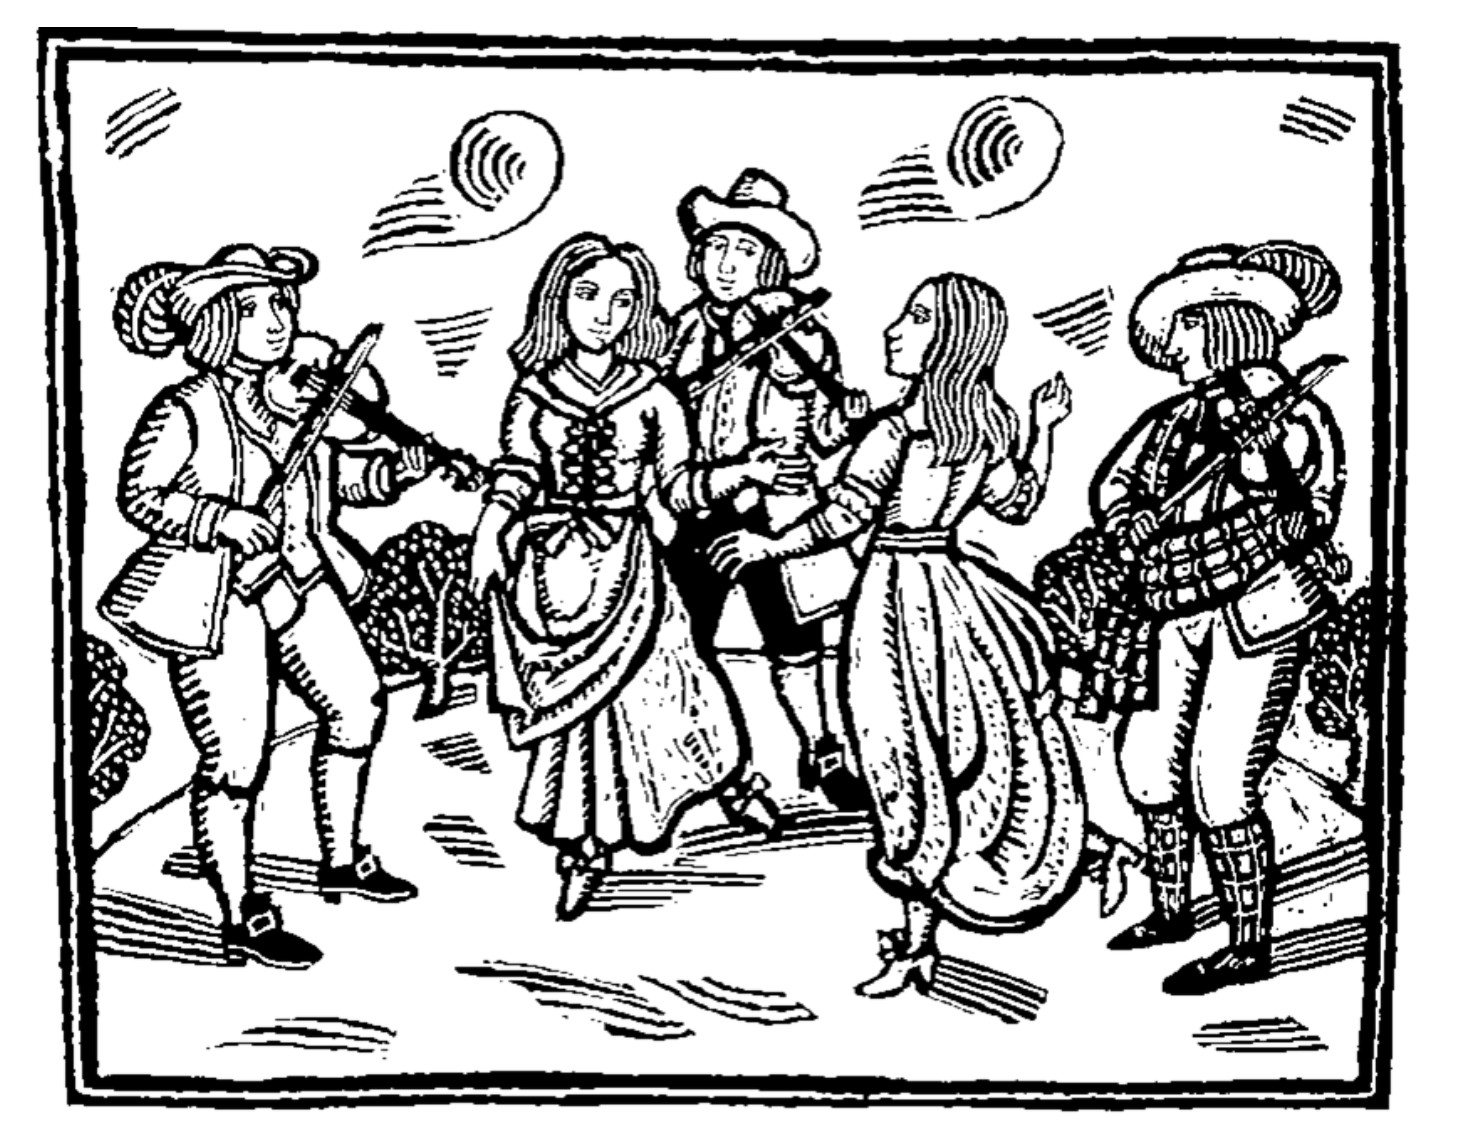
\includegraphics[width=8cm]{../images/reels}
\end{center}

\section{Irish Reels}
\begin{abc}[name=Cooleys]
X: 1
T: Cooley's
R: reel
M: 4/4
L: 1/8
K: Edor
|:GF|"Em"EBBA B2 EB|"Em"B2 AB "G"dBAG|"D"FDAD "G"BD"D"AD|"D"FDAD "Bm7"dAFD|
"Em"EBBA B2 EB|"Em"B2 AB "G"defg|"Bm"afec "Bm7"dBAF|"D"DEFD "Em"E2:|
|:gf|"Em"eB ~B2 efge|"Em"eB ~B2 "G"gedB|"D"A2 FA DAFA|"D"A2 FA "Bm"defg|
"Em"eB ~B2 eBgB|"Em"eB ~B2 "G"defg|"Bm"afec "Bm7"dBAF|"D"DEFD "Em"E2:|
\end{abc}

\begin{abc}[name=The_Drunken_Landlady]
X: 2
T: The Drunken Landlady
R: reel
M: 4/4
L: 1/8
K: Edor
dc | "Em"BE~E2 "Bm"BAFA|"Em"BE~E2 "Bm"BAFA|"A"ABAF "D"D2FD|"Bm"FA~A2 BAFA|
"Em"BE~E2 "Bm"BAFA|"Em"BE~E2 "Bm"BAFA|"A"A3B "Bm"dfec|"D"dBAF "Em"E2:|
|:FA | "Em"Beed e2de|"Bm"f2df efdB|"A"ABAF "D"D2FD|"D"FA~A2 "Bm"BAFA|
"Em"Beed "C"e2de|"Bm"f2df "A"efdB|"D"A3B "Bm"dfec|"Em"dBAF E2:|
\end{abc}

\begin{abc}[name=Toss_The_Feathers]
X: 3
T: Toss The Feathers
R: reel
M: 4/4
L: 1/8
V:1 name=melody clef=treble 
K: Edor
%1
[V:1]|:"Em"EB ~B2 dB ~B2|"Em"EBBA "D"FDFA|"Em"BE ~E2 BABd|[1"C"egfe "D"dBAF:|[2 "C"egfe "D"dBAe | 
%5
[V:1]"Em"Beed ((3efe) de|"Em"fede "Bm"fede|"Em"febe febe|"Em"fede "Bm"fede|
%9
[V:1]"Em"Beed ((3efe) de|"Bm"fede "D"defa|"G"b3 g "D"a3 f|"C"g2 fe "Bm"dBAF|
\end{abc}

\begin{abc}[name=Drowsy_Maggie]
X: 4
T: Drowsy Maggie
R: reel
M: 4/4
L: 1/8
K: Edor
|:"Em"E2BE dEBE|"Em"E2BE "D"AFDF|"Em"E2BE dEBE|[1"G"BABc "D"dAFD:|[2 "G"BABc "A7"dAFA|
"D"d2fd "A"c2ec|"D"defg afge|"D"d2fd "A"c2ec|"G"BABc "A7"dAFA|
"D"d2fd "A"c2ec|"D"defg afge|"A"afge "D"fdec|[1"G"BABc "D"dAFD:|[2"G"BABc "A7/E"dAFA |
\end{abc}

\begin{abc}[name=Hand_Me_Down_The_Tackle]
X: 5
T: Hand Me Down The Tackle
R: reel
M: 4/4
L: 1/8
K: Dmaj
|: "D"dD~D2 FAAB | "D"defd "G"edBc | "D"dD~D2 FAAF | "C"GFEF "A7"GABc |
"D"dD~D2 FAAB | "D"defd "A7"cdeg |"Bm"fdec "G"dcBA | "Em"GFEF "A7"GABc :|
"D"d2 fd Adfd | "D"~d2 fd "A"cdec | "D"d2 fd Adfd | "C"eEEF "A7"GABc |
"D"d2 fd Adfd | "D"d2 fd "A7"cdeg | "Bm"dfec "G"dcBA | "Em"GFEF "A7"GABc |
"D"d2 fd Adfd | "D"~d2 fd "A"cdec | "D"d2 fd Adfd | "Em"eEEF "A7"GAfg |
"D"~a3b afdf | "C"gfed "A7"ceag | "Bm"fdec "G"dcBA | "Em"GFEF "A7"GABc |
\end{abc}

\newpage
\section{Maggie's Pancakes}
\begin{abc}[name=Maggies_Pancakes]
X: 1
T: Maggie's Pancakes
R: reel
M: 4/4
L: 1/18
K: Dmaj
"Bm"fBB2 fgfe|"Bm"dB B1/2B1/2B GBdB|"A"cAA "D"dAA "A"ec|"A"AfdB ecAc|
"Bm"dB B1/2B1/2B fgfe|"G"dB B1/2B1/2B GBdB|"A"cABc ABc(e|"A"e)fec Bcde:|
"G"f2dB GBdB|"A"caec "Bm"dB B1/2B1/2B|"G"f2dB GBdB|"A"cAec Bcde|
"D"fd d1/2d1/2d fgfe|"G"dB B1/2B1/2B GBdB|"A"cA"D"dA "A"ecA(a|"A"a)fec Bcde:|
\end{abc}

\begin{abc}[name=The_Otters_Holt]
X: 2
T: The Otter's Holt
R: reel
M: 4/4
L: 1/8
K: Bmin
e|:"Bm"fBBA FEFB|"Bm"(3ABA FB "A"ABde|"G"fBBA FEFA|
"A"(3Bcd cA Bcde|"G"fBBA FEFB|"Bm"(3ABA FB "A"ABde|
"Bm"faaf "G"effe|1 "A"dBBA ~B3e:|2 "A"dBAF B3c|
|:"D"d2fd Adfa|"D"bfaf "G"effe|"D"d2fd Adfa|"G"bfaf "A"~e3f|
"D"~d2fd Adfa|"A"bfaf efde|"G"fBBA FEFA|1"A"(3Bcd cA ~B3c:|2"A"(3Bcd cA "Bm"~B3c|
\end{abc}

\begin{abc}[name=Hulls_Reel]
X: 3
T: Hull's Reel
R: reel
M: 4/4
L: 1/8
K: Emaj
"E"BEEc B2 Bc | "E"BEEB "A"cBce | "E"BEEc B2 GB | "A"cBce "B"fefg |
"E"BEEc B2 Bc | "E"BEEB cBce | "F#m"fgfe cagf |1 "A"eccB ceec :|2 "A"eccB ceef |
|: "E"gB (3BBB g2fe | "F#m"fc (3ccc c2 Bc | "A"fc (3ccc c2Bc | "E"eB (3BBB Bcef |
"C#m"gB (3BBB g2 fe | "F#m"fc (3ccc c2 ce | "A"fgfe cagf |1 "A"eccB ceef :|2 "A"eccB ceec |
\end{abc}

\begin{abc}[name=MacArthur_Road]
X: 4
T: MacArthur Road
R: reel
M: 4/4
L: 1/8
K: Emaj
|:"E"BG G1/2G1/2G Bcef|"E"g1/2g1/2g ge fece|"F#m"f3 g fece|"A"gefg fece|
"E"BG G1/2G1/2G Bcef|"C#m"f(gg)e fece|"A"f2 ge fece|1"B" Bcef e3 A:|2"B" Bcef "E"e3 g|
|:"E"be e1/2e1/2e be"A"c'e|"E"be e1/2e1/2e bgfe|"F#m"f2 fg fece|"A"aege fece|
|1"E"be e1/2e1/2e bec"A"'e|"E"be e1/2e1/2e bgfe|"A"f2 fg fecB|"B"Bcef "E"e3g:|
|2"E"BG G1/2G1/2G Bcef|"C#m"f(gg)e fece|"A"f2 ge fece|"B"Bcef "E"e4|
\end{abc}


\chapter{Hornpipes}
\begin{center}
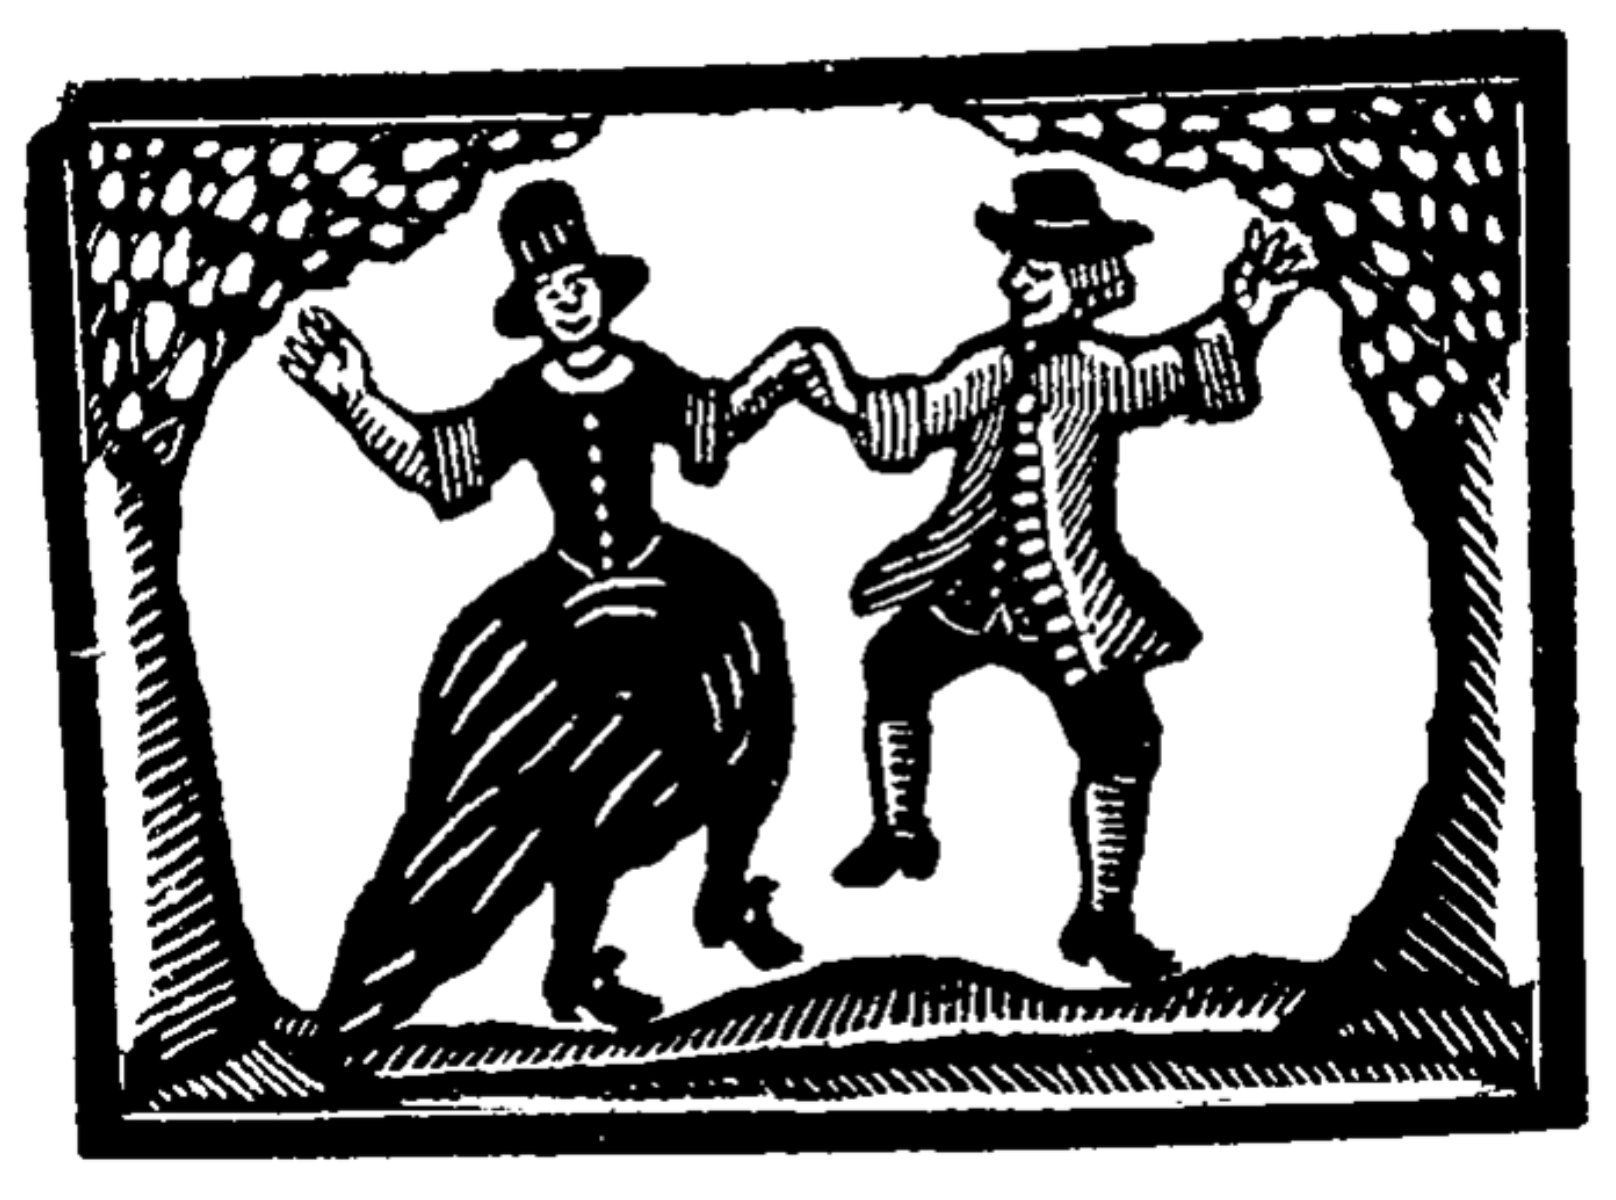
\includegraphics[width=8cm]{../images/hornpipes}
\end{center}

\chapter{Miscellaneous}
\begin{center}
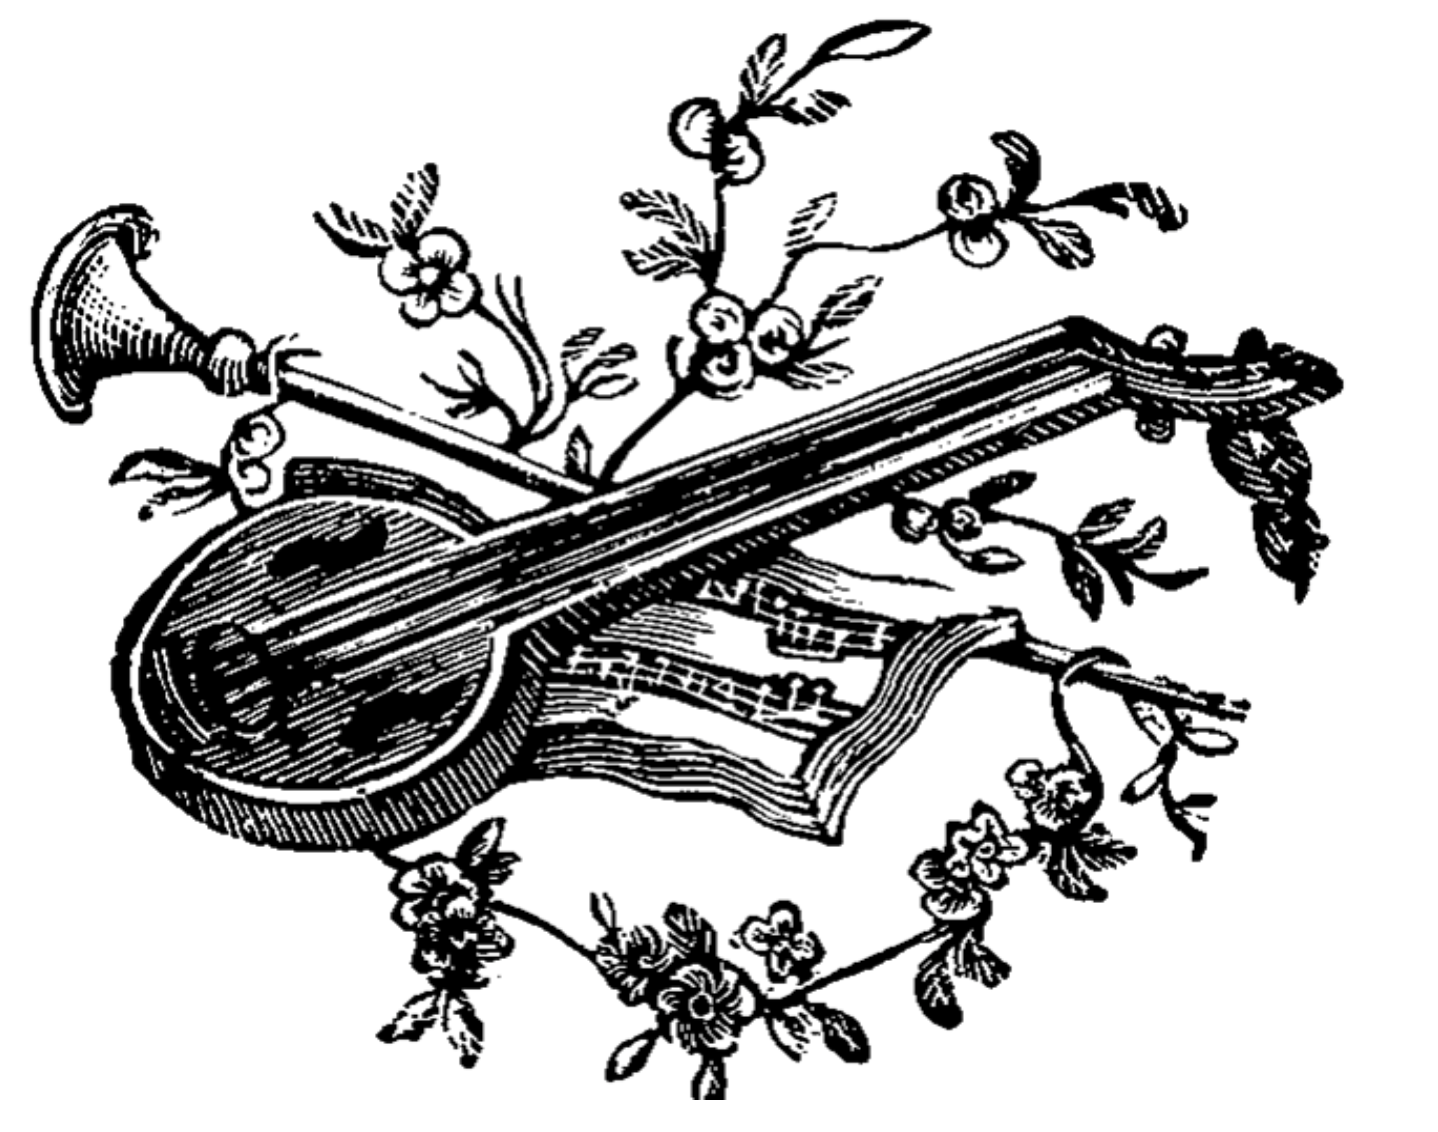
\includegraphics[width=8cm]{../images/misc}
\end{center}

\chapter{Waltzes}
\begin{center}
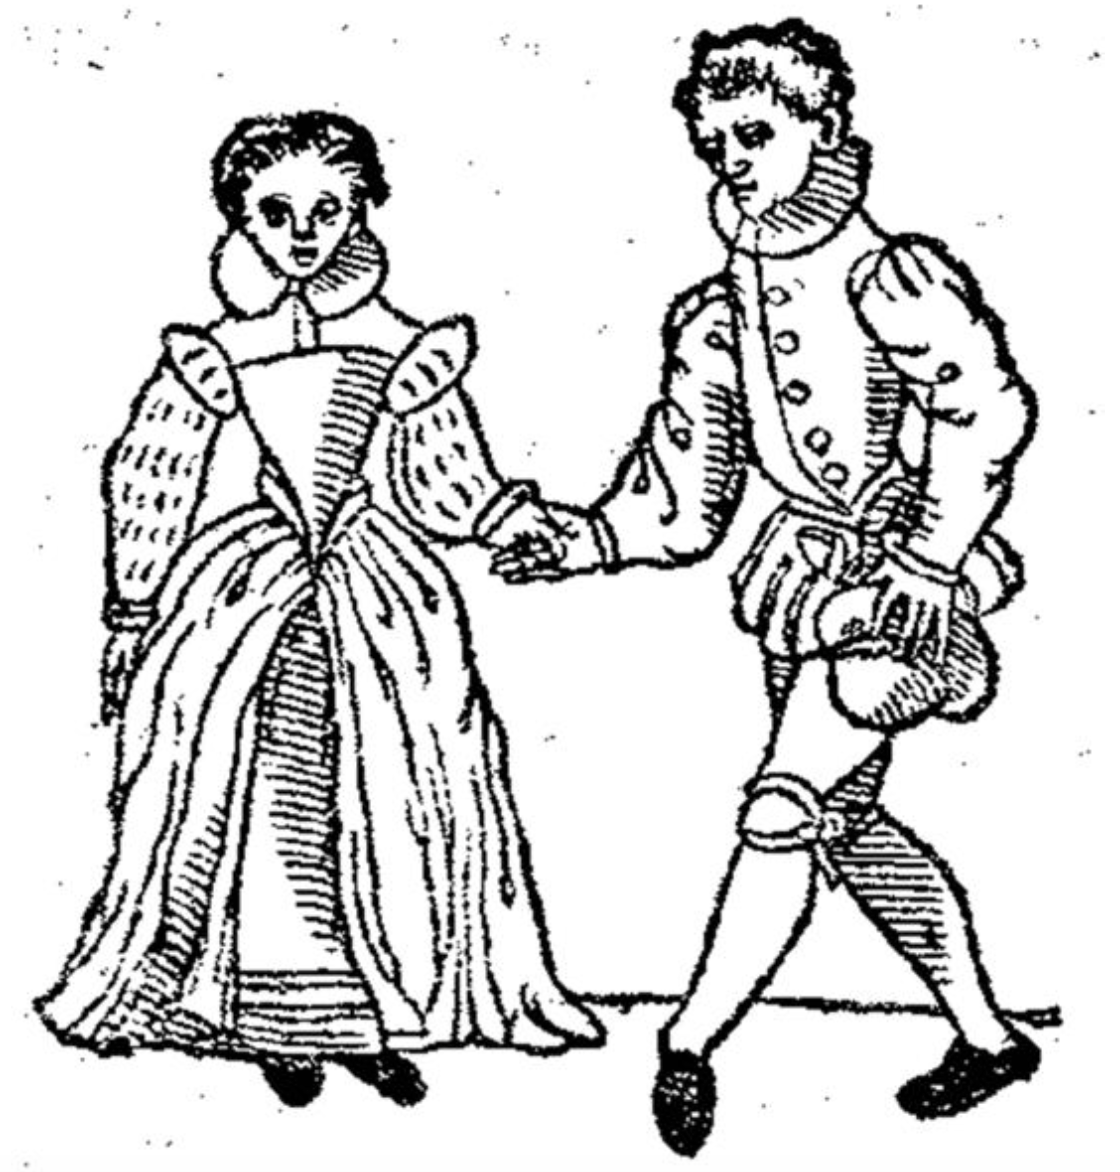
\includegraphics[width=8cm]{../images/waltzes}
\end{center}

%\section{Waltzes}
\section*{Margaret's}
\addcontentsline{toc}{section}{Margaret's}
\begin{abc}[name=Margarets]
X: 1
T: Margaret's
R: waltz
M: 3/4
L: 1/8
K: Gmaj
|: G>E | "G"D2- D>E G>A | "Em"B4 G>B | "C"A>G E2 G2 | "D"A4 (3AGE |
"G"D2- D>E G>A | "Em"B>c d2 G>A | "D(C)"B4 (3ABA | "G"G4 :|
B>c | "G"d2 e2 f2 | "C"g2 f2 g2 | "Am"e>d c2 e2 | "D"d4 B>A |
"G(Em)"G2- G>A Bc | "Bm"d2 B2 d2 | "C"e>d c2 (3BcB | "D"A4 (3ABc |
"G"d2 e2 f2 | "C"g>G f>G e>G | "G"d>G c>G B>G | "D"A4 (3AGE |
"G(Em)"D2 D>E G>A | "D(C)"B>d- d2 d>e | "(D)"B4 (3ABA | "G"G4 |]
\end{abc}

\section*{The Dark Island}
\addcontentsline{toc}{section}{The Dark Island}
\begin{abc}[name=The_Dark_Island]
X: 2
T: The Dark Island
R: waltz
M: 3/4
L: 1/8
K: Gmaj
|: E2 | "Dm" A3 E A2 | "Am" G3 A G2 | "F" E3 D C2 | "C" D4 GA |
[1 B3 A G2 | "Am" B d3 G2 | "C" B3 A G2 | "G" A4 :|
[2 "C" B3 D dB | "G7" A3 D BA | "C" G6 | G4 |]
Bc | "C" d3 B d2 | B3 A G2 | "F" E3 C E2 | "C" D4 GA | B3 A G2 |
"Am" B d3 GA | "C" B3 A G2 | "G" A4 EG | "Dm" A4 A2 | "Am" G4 G2 |
"F" E3 D C2 | "C" D4 GA | B3 D dB | "G7" A3 D BA | "C" G6 | G6 |]
\end{abc}

\section*{Carolan's Welcome}
\addcontentsline{toc}{section}{Carolan's Welcome}
\begin{abc}[name=Carolans_Welcome1]
X: 3
T: Carolan's Welcome Pt.1
R: waltz
M: 3/4
L: 1/8
K: Bmin
V:1
dc|:B2 de f2|B2 de f2|ef ed cB|(3ABc A2 F2|
V:2
dc|:B3c d2|d3c B2|c3d cB|A4 F2|
V:1
d3c B2|e3d c2|df F2 A2|B4 dc|
V:2
d3A GF|G3A Bc|d3d cd|B4 dc|
V:1
B2 de f2|B2 de f2|ef ed cB|(3ABc A2 F2|
V:2
B3c d2|d3c B2|c3d cB|A4 F2|
V:1
a3g f2|b3a fe|df ed cd|[1 B4 dc :|[2 B4 B2|]
V:2
d6|e6|d4 cd|[1B6:|[2B6|]
\end{abc}
\begin{abc}[name=Carolans_Welcome2]
X: 3
T: Carolan's Welcome Pt.2
R: waltz
M: 3/4
L: 1/8
K: Bmin
V:1
|:F2 Bc d2|F2 Bc d2|dc BA Bc|d2 F2 F2|
V:2
|:B6|B6|B6|A6|
V:1
g2 bg fe|f2 af ed|e2 f2 a2|b6|
V:2
e6|d6|c6|dc BA FA|
V:1
ba fa b2|afef a2|fe de fd|e2 c2 (3ABc|
V:2
g6|f6|d6|cd ef ge|
V:1
d3c B2|e3d c2|df F2 A2|[1 B4 B2 :|[2 B6|]
V:2
fe dc df|GF GA Bc|d4 cd|[1B6:|[2 B6|]
\end{abc}

\section*{Ashokan Farewell}
\addcontentsline{toc}{section}{Ashokan Farewell}
\begin{abc}[name=Ashokan_Farewell]
X: 4
T: Ashokan Farewell
R: waltz
M: 3/4
L: 1/8
K: Dmaj
Ac|:"D" d3 cBA|"D7" F4 EF|"G" G3 FED|"Em" B,2D3B,|
"D" A,2D2F2|"Bm" A2d2f2|"Em" f3gf2|"A7" e4Acj|
"D" d3 cBA|"F#m" F4 EF|"G" G3 FED|"Em" B,2D3B,|
"D" A,2D2F2|"Bm" A2d2f2|"A7" A2c2e2|1"D" d4Ac:|2"D" d4FG|]
|:"D" A3FD2|"D7" d4A2|"G" B3cd2|"D" AF3E2|
"D" F3ED2|"Bm" B,4?G,2|"A" A,6|"A7" A4 FE|
"D" D2F2A2|"C" =c6|"G" B3cd2|"D" AF3D2|
"D" A,2D2F2|"Bm" A2d2F2|"Em" E3D"A7"C2|1"D"D4FG:|2"D" D6|]
\end{abc}

\section*{Flatbush}
\addcontentsline{toc}{section}{Flatbush}
\begin{abc}[name=Flatbush]
X: 5
T: Flatbush
R: waltz
M: 3/4
L: 1/8
K: Emin
| "Em"B3 eBA | G2 E2 E2 | B3 eBG | "Am"A3 c BA |
 "Em"EF GA BG/2B/2 | "Am"A/2B/2E A2 A2 | "Em"G3 A"F"=FG | "Em"E EGBeG |
 "Em"[B3 E3] [eB][BG][AF]| [G2E2] [E2B,2] [E2B,2] | [B3G3] [eB][BG][GE] | "Am"A3 d (3cBA |
 "G"GA Bc dB | "Am"A/2B/2E A2 A2 | "Em"G3 A"F"=FG | "Em"E6 |
 "Em"[g4B4] [fA][eG] | "B"[fA] B,DFBd | "C"[e2G2] [d3F3][cE] | "G"[B6D6] |
 "Am"[c2E2] [B2D2] [A2C2] | "Em"[B2D2] [e2G2] [f2A2] | [g3B3] [fA][gB][ac] | "B7"[f6A6] |
 "Em"[g4B4] [fA][eG] | "B"[fA] B,DFBd | "C"[e2G2] [d3F3][cE] | "G"[B6D6] |
 "Am"[c2E2] [B2D2] [A2C2] | "Em"[B2D2] [e2G2] [f2A2] | [g3B3] [aA]"F"=[fF][gG]| "Em"[e6E6] |]
\end{abc}

\end{document}